% Options for packages loaded elsewhere
\PassOptionsToPackage{unicode}{hyperref}
\PassOptionsToPackage{hyphens}{url}
\PassOptionsToPackage{dvipsnames,svgnames,x11names}{xcolor}
%
\documentclass[
  letterpaper,
  DIV=11,
  numbers=noendperiod]{scrartcl}

\usepackage{amsmath,amssymb}
\usepackage{iftex}
\ifPDFTeX
  \usepackage[T1]{fontenc}
  \usepackage[utf8]{inputenc}
  \usepackage{textcomp} % provide euro and other symbols
\else % if luatex or xetex
  \usepackage{unicode-math}
  \defaultfontfeatures{Scale=MatchLowercase}
  \defaultfontfeatures[\rmfamily]{Ligatures=TeX,Scale=1}
\fi
\usepackage{lmodern}
\ifPDFTeX\else  
    % xetex/luatex font selection
\fi
% Use upquote if available, for straight quotes in verbatim environments
\IfFileExists{upquote.sty}{\usepackage{upquote}}{}
\IfFileExists{microtype.sty}{% use microtype if available
  \usepackage[]{microtype}
  \UseMicrotypeSet[protrusion]{basicmath} % disable protrusion for tt fonts
}{}
\makeatletter
\@ifundefined{KOMAClassName}{% if non-KOMA class
  \IfFileExists{parskip.sty}{%
    \usepackage{parskip}
  }{% else
    \setlength{\parindent}{0pt}
    \setlength{\parskip}{6pt plus 2pt minus 1pt}}
}{% if KOMA class
  \KOMAoptions{parskip=half}}
\makeatother
\usepackage{xcolor}
\setlength{\emergencystretch}{3em} % prevent overfull lines
\setcounter{secnumdepth}{-\maxdimen} % remove section numbering
% Make \paragraph and \subparagraph free-standing
\makeatletter
\ifx\paragraph\undefined\else
  \let\oldparagraph\paragraph
  \renewcommand{\paragraph}{
    \@ifstar
      \xxxParagraphStar
      \xxxParagraphNoStar
  }
  \newcommand{\xxxParagraphStar}[1]{\oldparagraph*{#1}\mbox{}}
  \newcommand{\xxxParagraphNoStar}[1]{\oldparagraph{#1}\mbox{}}
\fi
\ifx\subparagraph\undefined\else
  \let\oldsubparagraph\subparagraph
  \renewcommand{\subparagraph}{
    \@ifstar
      \xxxSubParagraphStar
      \xxxSubParagraphNoStar
  }
  \newcommand{\xxxSubParagraphStar}[1]{\oldsubparagraph*{#1}\mbox{}}
  \newcommand{\xxxSubParagraphNoStar}[1]{\oldsubparagraph{#1}\mbox{}}
\fi
\makeatother


\providecommand{\tightlist}{%
  \setlength{\itemsep}{0pt}\setlength{\parskip}{0pt}}\usepackage{longtable,booktabs,array}
\usepackage{calc} % for calculating minipage widths
% Correct order of tables after \paragraph or \subparagraph
\usepackage{etoolbox}
\makeatletter
\patchcmd\longtable{\par}{\if@noskipsec\mbox{}\fi\par}{}{}
\makeatother
% Allow footnotes in longtable head/foot
\IfFileExists{footnotehyper.sty}{\usepackage{footnotehyper}}{\usepackage{footnote}}
\makesavenoteenv{longtable}
\usepackage{graphicx}
\makeatletter
\def\maxwidth{\ifdim\Gin@nat@width>\linewidth\linewidth\else\Gin@nat@width\fi}
\def\maxheight{\ifdim\Gin@nat@height>\textheight\textheight\else\Gin@nat@height\fi}
\makeatother
% Scale images if necessary, so that they will not overflow the page
% margins by default, and it is still possible to overwrite the defaults
% using explicit options in \includegraphics[width, height, ...]{}
\setkeys{Gin}{width=\maxwidth,height=\maxheight,keepaspectratio}
% Set default figure placement to htbp
\makeatletter
\def\fps@figure{htbp}
\makeatother

\KOMAoption{captions}{tableheading}
\makeatletter
\@ifpackageloaded{tcolorbox}{}{\usepackage[skins,breakable]{tcolorbox}}
\@ifpackageloaded{fontawesome5}{}{\usepackage{fontawesome5}}
\definecolor{quarto-callout-color}{HTML}{909090}
\definecolor{quarto-callout-note-color}{HTML}{0758E5}
\definecolor{quarto-callout-important-color}{HTML}{CC1914}
\definecolor{quarto-callout-warning-color}{HTML}{EB9113}
\definecolor{quarto-callout-tip-color}{HTML}{00A047}
\definecolor{quarto-callout-caution-color}{HTML}{FC5300}
\definecolor{quarto-callout-color-frame}{HTML}{acacac}
\definecolor{quarto-callout-note-color-frame}{HTML}{4582ec}
\definecolor{quarto-callout-important-color-frame}{HTML}{d9534f}
\definecolor{quarto-callout-warning-color-frame}{HTML}{f0ad4e}
\definecolor{quarto-callout-tip-color-frame}{HTML}{02b875}
\definecolor{quarto-callout-caution-color-frame}{HTML}{fd7e14}
\makeatother
\makeatletter
\@ifpackageloaded{caption}{}{\usepackage{caption}}
\AtBeginDocument{%
\ifdefined\contentsname
  \renewcommand*\contentsname{Table of contents}
\else
  \newcommand\contentsname{Table of contents}
\fi
\ifdefined\listfigurename
  \renewcommand*\listfigurename{List of Figures}
\else
  \newcommand\listfigurename{List of Figures}
\fi
\ifdefined\listtablename
  \renewcommand*\listtablename{List of Tables}
\else
  \newcommand\listtablename{List of Tables}
\fi
\ifdefined\figurename
  \renewcommand*\figurename{Figure}
\else
  \newcommand\figurename{Figure}
\fi
\ifdefined\tablename
  \renewcommand*\tablename{Table}
\else
  \newcommand\tablename{Table}
\fi
}
\@ifpackageloaded{float}{}{\usepackage{float}}
\floatstyle{ruled}
\@ifundefined{c@chapter}{\newfloat{codelisting}{h}{lop}}{\newfloat{codelisting}{h}{lop}[chapter]}
\floatname{codelisting}{Listing}
\newcommand*\listoflistings{\listof{codelisting}{List of Listings}}
\makeatother
\makeatletter
\makeatother
\makeatletter
\@ifpackageloaded{caption}{}{\usepackage{caption}}
\@ifpackageloaded{subcaption}{}{\usepackage{subcaption}}
\makeatother
\makeatletter
\@ifpackageloaded{fontawesome5}{}{\usepackage{fontawesome5}}
\makeatother

\ifLuaTeX
  \usepackage{selnolig}  % disable illegal ligatures
\fi
\usepackage{bookmark}

\IfFileExists{xurl.sty}{\usepackage{xurl}}{} % add URL line breaks if available
\urlstyle{same} % disable monospaced font for URLs
\hypersetup{
  pdftitle={Lab 1: Introduction},
  pdfauthor={Shunkei Kakimoto},
  colorlinks=true,
  linkcolor={blue},
  filecolor={Maroon},
  citecolor={Blue},
  urlcolor={Blue},
  pdfcreator={LaTeX via pandoc}}


\title{Lab 1: Introduction}
\usepackage{etoolbox}
\makeatletter
\providecommand{\subtitle}[1]{% add subtitle to \maketitle
  \apptocmd{\@title}{\par {\large #1 \par}}{}{}
}
\makeatother
\subtitle{APEC 1101 - Applied Economics, University of Minnesota}
\author{Shunkei Kakimoto}
\date{}

\begin{document}
\maketitle


\subsection{\texorpdfstring{\faIcon{list}
Outline}{ Outline}}\label{outline}

\begin{itemize}
\tightlist
\item
  About Myself
\item
  Some Important Information
\item
  Introduction to Economic Way of Thinking
\end{itemize}

\subsection{About Myself}\label{about-myself}

\begin{itemize}
\tightlist
\item
  \textbf{Shunkei Kakimoto}
\item
  from Japan
\item
  3rd year Ph.D.~in Applied Economics
\end{itemize}

\begin{itemize}
\tightlist
\item
  I was a TA in Econometrics and Microeconomics for Ph.D.
\item
  First time teaching Microeconomics to undergraudate students!
\end{itemize}

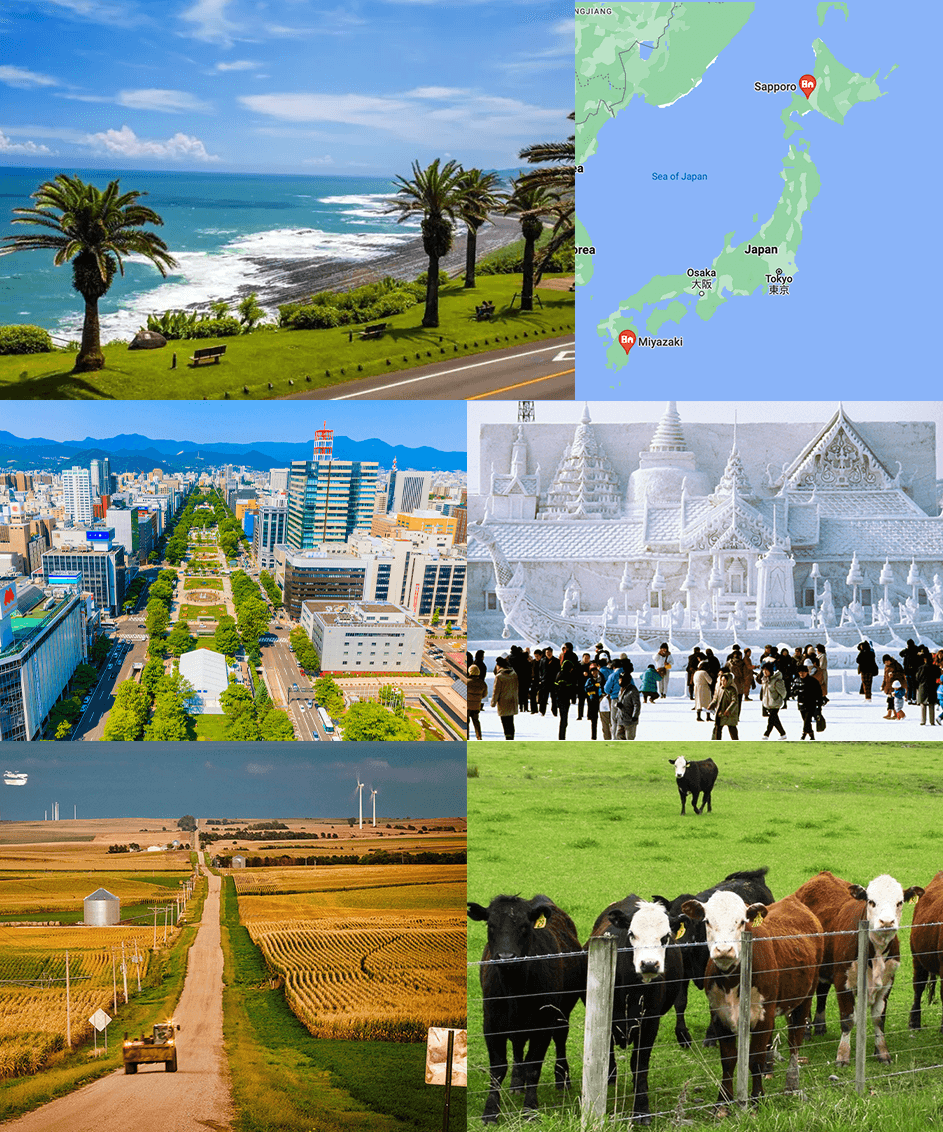
\includegraphics[width=0.7\textwidth,height=\textheight]{image/pictures.png}

\subsection{Contact Infomation}\label{contact-infomation}

\begin{itemize}
\tightlist
\item
  \faIcon{envelope} \textbf{Email}: kakim002@umn.edu

  \begin{itemize}
  \tightlist
  \item
    Feel free to shoot me an email if you have any questions or
    concerns. I'll get back to you as soon as possible.
  \end{itemize}
\item
  \faIcon{building-columns} \textbf{Office}: 316a Ruttan Hall
\end{itemize}

\begin{itemize}
\tightlist
\item
  \textbf{Office hours in Waite Library}:

  \begin{itemize}
  \tightlist
  \item
    Tuesday 1:00-2:00 pm
  \item
    Thursday 1:00-2:00 pm
  \item
    Or by appointment (email me)
  \end{itemize}
\end{itemize}

\subsection{Assignment Procedure}\label{assignment-procedure}

You have two options to submit your assignments:

\begin{itemize}
\tightlist
\item
  \textbf{Option 1}: Submit a physical copy of your assignment in person
  during class.
\item
  \textbf{Option 2}: Send me your assignment (e.g., pdf) by email
  (Please CC Tade)
\end{itemize}

\begin{tcolorbox}[enhanced jigsaw, left=2mm, bottomrule=.15mm, rightrule=.15mm, colback=white, title=\textcolor{quarto-callout-caution-color}{\faFire}\hspace{0.5em}{Please make sure to:}, colbacktitle=quarto-callout-caution-color!10!white, toprule=.15mm, colframe=quarto-callout-caution-color-frame, titlerule=0mm, bottomtitle=1mm, toptitle=1mm, arc=.35mm, breakable, opacityback=0, leftrule=.75mm, opacitybacktitle=0.6, coltitle=black]

\begin{itemize}
\tightlist
\item
  When you submit your assignments by email, please make it {\textbf{one
  single PDF file}} (please do not send multiple files).
\end{itemize}

\end{tcolorbox}

\begin{tcolorbox}[enhanced jigsaw, left=2mm, bottomrule=.15mm, rightrule=.15mm, colback=white, title=\textcolor{quarto-callout-important-color}{\faExclamation}\hspace{0.5em}{Syllabus is important!}, colbacktitle=quarto-callout-important-color!10!white, toprule=.15mm, colframe=quarto-callout-important-color-frame, titlerule=0mm, bottomtitle=1mm, toptitle=1mm, arc=.35mm, breakable, opacityback=0, leftrule=.75mm, opacitybacktitle=0.6, coltitle=black]

Please read the syllabus carefully. It contains important information
about the course, including the grading policy, assignment due dates,
the course content, and the schedule.

\end{tcolorbox}

\begin{itemize}
\item
  The syllabus is important because it contains important information
  about the course, including the grading policy, assignment due dates,
  the course content, and the schedule.
\item
  It's like a rule book for the course.
\item
  I am here to help you succeed in this course. I want to you help you
  out if you are having a difficult time. So, please don't hesitate to
  reach out to me if you have any questions or concerns.
\end{itemize}

\section{Introduction}\label{introduction}

\subsection{}\label{section}

Learning Objectives of This Course

To introduce you to \textbf{the economic way of thinking} and
\textbf{how to apply it to real-world problems}:

Specifically, there are two key components to achieve this goal:

\begin{enumerate}
\def\labelenumi{\arabic{enumi}.}
\tightlist
\item
  obtain the fundamental knowledge of microeconomic theories and
  concepts.
\item
  learn the skills to apply these concepts to real-world problems.
\end{enumerate}

What is the economic way of thinking?

\begin{itemize}
\tightlist
\item
  In this course, we will learn about the basic principles of economics.
  Let me clarify the course objectives, which is very important.
\item
  As written on the syllabus, the objective of this course is to
  introduce you to the economic way of thinking and how to apply it to
  real-world problems.
\end{itemize}

\begin{itemize}
\tightlist
\item
  In this course, we will learn about the basic principles of economics.
\item
  What is economics? Why is it important?
\item
  Regardless of your major, economics is a useful tool for understanding
  the world around you.
\item
  Let me talk about the field of economics, and the importance of
  economics.
\end{itemize}

\subsection{What is the economics way of
thinking?}\label{what-is-the-economics-way-of-thinking}

\subsubsection{Example 1: Trade-offs in Everyday
Life}\label{example-1-trade-offs-in-everyday-life}

It's Friday night, and you order a pizza. You are really hungry so you
ate most of it (it was so delicious), there are only two slices left.

Should you eat them now or save them for tomorrow?

Question

What is the trade-off here?


\includegraphics[width=0.6\textwidth,height=\textheight]{lab1_files/mediabag/view-cartoon-waiter-.jpg}

\subsection{What is the economics way of
thinking?}\label{what-is-the-economics-way-of-thinking-1}

\subsubsection{Example 2: Groundwater
Pollution}\label{example-2-groundwater-pollution}

In the Midwest region, there is a serious problem of groundwater
pollution due to the excessive use of fertilizers. Because of this, the
water quality in the surrounding residential has been deteriorating,
causing health problems for the residents.

{How should we address this problem?}

\begin{figure}[H]

{\centering 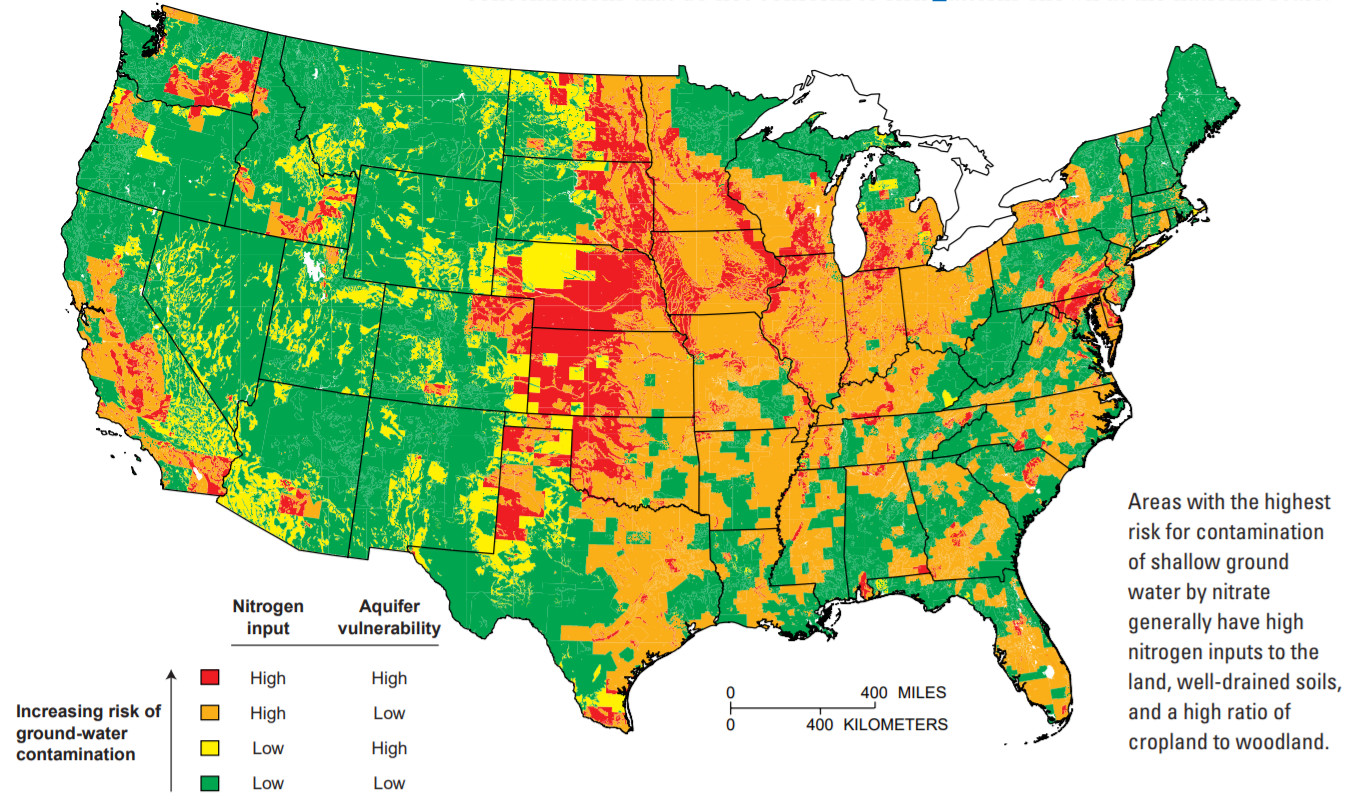
\includegraphics{lab1_files/mediabag/wss-nitrogen-map-us-.jpg}

}

\caption{Figure: Areas at high risk of nitrogen contamination of
groundwater(Reference:
\href{https://www.usgs.gov/media/images/areas-high-risk-nitrogen-contamination-groundwater}{USGS})}

\end{figure}%

\begin{itemize}
\item
  Trade-offs are everywhere in our daily lives, and it's the most
  fundamental concept in economics. Basically, we want to solve the
  trade-offs to achieve a better outcome.
\item
  Meanwhile, sometime, trade-off can be used to solve the problem.
\item
  The problem of the groundwater pollution is a typical example of the
  trade-off. Assuming that the farmers are pursuing their own profits,
  they will use whatever amount of fertilizers they need to maximize
  their profits. However, this will lead to the groundwater pollution.
\item
  What is the solution for this problem?
\item
  We can use the melanism of trade-off to solve this problem. For
  example, we can impose a tax on the use of fertilizers. This will
  increase the cost of using fertilizers, and the farmers will reduce
  the use of fertilizers. This will reduce the groundwater pollution.
\item
  Or, we can subsidize the farmers to reduce the use of fertilizers.
  This will also reduce the groundwater pollution.
\item
  Which is economically efficient?
\end{itemize}




\end{document}
